\documentclass[a0,portrait]{a0poster}

\usepackage{setspace}
\usepackage[scaled]{beramono}
\usepackage[utf8]{inputenc}
\usepackage[tabular,lining]{montserrat}
\renewcommand*\familydefault{\sfdefault}
\usepackage[T1]{fontenc}
\usepackage[portuges]{babel}
\usepackage{amsfonts, amsmath, amsthm, amssymb}
\usepackage{graphicx, url, float, booktabs, datetime, multicol}
\usepackage{lipsum, cite, wrapfig}
\usepackage[hang]{subfig}
\usepackage[font=large,labelfont=bf]{caption}
\usepackage[ruled]{algorithm2e}
\usepackage[super]{nth}
\usepackage[hang]{subfig}
\usepackage[svgnames]{xcolor} % Specify colors by their 'svgnames', for a full list of all colors available see here: http://www.latextemplates.com/svgnames-colors
\usepackage[
    breaklinks=true,    
    allbordercolors=Indigo,
%    ocgcolorlinks=true,
    colorlinks=true,
    anchorcolor=Indigo, 
    citecolor=black,
    filecolor=Indigo,
    linkcolor=Indigo,
    menucolor=Indigo,
    runcolor=Indigo,
    urlcolor=Indigo,
    linktoc=all
]{hyperref}
\usepackage[ocgcolorlinks]{ocgx2}

\usepackage{pgf}
\usepackage{pgfpages}

\pgfpagesdeclarelayout{boxed}
{
  \edef\pgfpageoptionborder{0pt}
}
{
  \pgfpagesphysicalpageoptions
  {%
    logical pages=1,%
  }
  \pgfpageslogicalpageoptions{1}
  {
      border code=\pgfsetlinewidth{4pt}\color{Indigo}\pgfstroke,%
    border shrink=\pgfpageoptionborder,%
    resized width=.95\pgfphysicalwidth,%
    resized height=.95\pgfphysicalheight,%
    center=\pgfpoint{.5\pgfphysicalwidth}{.5\pgfphysicalheight}%
  }%
}

\pgfpagesuselayout{boxed}

\columnsep=100pt
\columnseprule=4pt

\usepackage{sectsty}
\usepackage[most]{tcolorbox}

\tcbset{
    frame code={}
    center title,
    left=0pt,
    right=0pt,
    top=0pt,
    bottom=0pt,
    colback=Indigo!10,
    colframe=black,
    width=\dimexpr\linewidth\relax,
    enlarge left by=0mm,
    boxsep=3pt,
    arc=0pt,outer arc=0pt,
    }


\usepackage{tikz}
    \usetikzlibrary{positioning}
    \usetikzlibrary{arrows}

\tikzset{basic/.style={draw,fill=Gray!50,text width=1em,text badly centered}}
\tikzset{input/.style={basic,circle}}
\tikzset{weights/.style={basic,rectangle}}
\tikzset{functions/.style={basic,circle,fill=Gray!25}}
\tikzset{int/.style={draw, fill=Gray!50, minimum size=2em}}

% \allsectionfont{\fontfamily{Montserrat-TOsF}}

\setlength\parindent{5cm}

\begin{document}

    \noindent
\begin{minipage}{0.73\linewidth}
    % \headingfont
\veryHuge \color{Indigo} \textbf{Fundamentos de Redes Neurais Profundas:}\\ \color{Black}
\Huge\textit{Abordagem Baseada em Redes Convolucionais.}\\[1cm] % Subtitle
\huge \textbf{Rafael Gonçalves \& Romis Attux.}\\[0.2cm] % Author(s)
    {\LARGE Faculdade de Engenharia Elétrica e de Computação - Unicamp\\
    \texttt{r186062@dac.unicamp.br, attux@dca.fee.unicamp.br}}
\end{minipage}
%
\begin{minipage}{0.27\linewidth}
    \centering
    \vspace{2cm}
    \def\svgwidth{0.6\columnwidth}
    \input{unicamp.pdf_tex}
    \break\hfill\break
\end{minipage}

\vspace{1cm} % A bit of extra whitespace between the header and poster content

\begin{multicols}{2}

\onehalfspacing
    \section*{\begin{tcolorbox}
        \huge
        % \headingfont
        \centering
        Introdução
    \end{tcolorbox}}

\Large

    Redes neurais artificiais são sistemas de computação não lineares e adaptativos originalmente inspirados nas redes neurais biológicas presentes no sistema nervoso dos animais.
    Especialmente com o advento de redes neurais profundas e o conceito de aprendizado profundo, este se tornou um importante paradigma dentro do campo de aprendizado de máquina e é amplamente utilizado para resolver uma variedade de problemas atuais.

    Neste contexto, esta pesquisa buscou estudar teoricamente redes neurais profundas baseado em um livro recente e representativo ~\cite{Goodfellow16} e posteriormente aplicar um modelo específico de rede neural -- a saber uma rede convolucional -- ao problema conhecido de reconhecimento de dígitos escritos à mão utilizando a base de dados MNIST ~\cite{mnist}.

    \section*{\begin{tcolorbox}
        \huge
        % \headingfont
        \centering
        Discussões e Resultados
    \end{tcolorbox}}
    \Large

    \subsection*{\LARGE\color{Indigo}MLP}

\begin{figure}[H]
\centering
    \begin{tikzpicture}[>=latex']
        \node[functions] (center) {};
        \node[below of=center,font=\scriptsize,text width=4em] {activation function};
        \draw[very thick] (0em,0em) -- (-0.8em,0em);
        \draw[very thick] (0em,0em) -- (0.70em,0.70em);
        \draw[very thin] (0em,0.75em) -- (0em,-0.75em);
        \draw[very thin] (0.75em,0em) -- (-0.75em,0em);
        \node[right of=center] (right) {};
            \path[draw,->] (center) -- (right);
        \node[functions,left=3em of center] (left) {$\sum$};
            \path[draw,->] (left) -- (center);
        \node[weights,left=3em of left] (2) {$w_2$} -- (2) node[input,left of=2, left=1em] (l2) {$x_2$};
            \path[draw,->] (l2) -- (2);
            \path[draw,->] (2) -- (left);
        \node[below of=2] (dots) {$\vdots$} -- (dots) node[left of=dots, left=1em] (ldots) {$\vdots$};
        \node[weights,below of=dots] (n) {$w_n$} -- (n) node[input,left of=n, left=1em] (ln) {$x_n$};
            \path[draw,->] (ln) -- (n);
            \path[draw,->] (n) -- (left);
        \node[weights,above of=2] (1) {$w_1$} -- (1) node[input,left of=1, left=1em] (l1) {$x_1$};
            \path[draw,->] (l1) -- (1);
            \path[draw,->] (1) -- (left);
        \node[weights,above of=1] (0) {$w_0$} -- (0) node[input,left of=0, left=1em] (l0) {$1$};
            \path[draw,->] (l0) -- (0);
            \path[draw,->] (0) -- (left);
        \node[below of=ln,font=\scriptsize] {inputs};
        \node[below of=n,font=\scriptsize] {weights};
    \end{tikzpicture}
    \caption{Neurônio perceptron.}
\label{fig:perc}\par
\end{figure}

As redes MLP podem ser vistas como redes de neurônios perceptron interligados em forma de camadas: uma camada de entrada que recebe cada entrada do vetor $\mathbf{x}$, uma ou mais camadas intermediárias e uma camada de saída. Exemplo de uma rede MLP pode ser visto na figura ~\ref{fig:mlp}.

  \begin{figure}[H]
        {\centering
        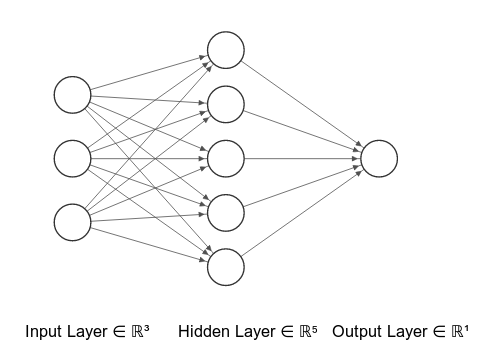
\includegraphics[width=.6\linewidth]{mlp_ex.png}
        \caption{Exemplo de rede MLP com 3 atributos de entrada, uma camada intermediária com 5 neurônios e uma camada de saída com um único neurônio, gerado com ~\cite{nnsvg}.}
        \label{fig:mlp}\par}
  \end{figure}

  Desta forma, matematicamente a saída de uma dessas redes -- considerando $\mathbf{W^n}$ e $f^n$ como respectivamente matriz de pesos e função de ativação da camada n --  é:

  $$
  y = f^N(\mathbf{W^N}\cdot ... f^2(\mathbf{W^2}\cdot f^1(\mathbf{W^1} \cdot \mathbf{x} + w_0^1) + w_0^2) + w_0^N)
  $$

  Ou ainda se definirmos uma matriz de entrada que admita $M$ exemplos em uma mesma estrutura:

\begin{equation}
    \label{eq:mlp}
  \mathbf{y} = \mathbf{F^n}( ... \mathbf{F^2}(\mathbf{F^1}(\boldsymbol{\Phi} \cdot \mathbf{W^1})\mathbf{W^2})\mathbf{W^N})
\end{equation}

  Com:

\hfill
$
\mathbf{X} =\begin{bmatrix}
    \mathbf{x_1} \\
    \mathbf{x_2} \\
    \vdots \\
    \mathbf{x_M}
\end{bmatrix}
$
\hfill
$
\boldsymbol{\Phi} = \boldsymbol{\Phi}(\mathbf{X}) = \begin{bmatrix}
    1 & \mathbf{x_1} \\
    1 & \mathbf{x_2} \\
    &\vdots \\
    1 & \mathbf{x_M}
\end{bmatrix}
$
\hfill
$
\mathbf{y} =\begin{bmatrix}
    y_1 \\
    y_2 \\
    \vdots \\
    y_M
\end{bmatrix}
$
\hfill
\break

$$
\mathbf{{F^n}(u)} = 
\begin{bmatrix}
  f^n(u_1) & 0 & \cdots  & 0 \\
  0 & f^n(u_2) & \cdots  & 0 \\
  \vdots   & \vdots & \ddots & \vdots \\
  0 & 0 & \cdots  & f^n(u_M) \\
\end{bmatrix}
$$
    \subsection*{\LARGE\color{Indigo}CNN}
    
\begin{figure}[H]
    {\centering
    \begin{tikzpicture}[node distance=10em,auto,>=latex']
        \node [int] (a) {Convolution};
        \node [int] (c) [right of=a] {Activation};
        \node [int] (e) [right of=c] {Pooling};
        \path[draw,->] (a) -- (c);
        \path[draw,->] (c) -- (e);
    \end{tikzpicture}
    \caption{Etapas de uma camada convolucional.}
    \label{fig:conv}\par}
\end{figure}


  Exemplo da operação de convolução entre uma imagem $\mathbf{I}$ 2D e um kernel $\mathbf{K}$~\cite{ia006}:

\begin{equation}
  (I*K)(i, j) = (K*I)(i,j) = \sum_m\sum_n K(m, n) \cdot I(i-m, j-n)
\end{equation}

A figura ~\ref{fig:cnn} mostra um exemplo de CNN.

  \begin{figure}[H]
        {\centering
        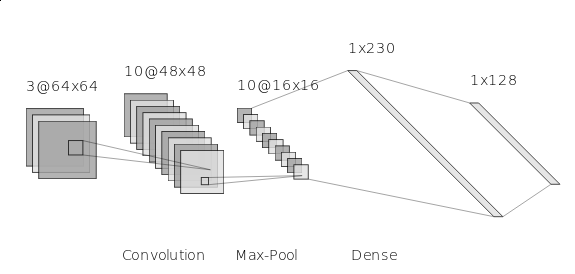
\includegraphics[width=\linewidth]{cnn_ex.png}
        \caption{Exemplo de rede CNN com 1 camada convolucional - convolução e max-polling - e 2 camadas FC, gerado com ~\cite{nnsvg}.}
        \label{fig:cnn}\par}
  \end{figure}

  \begin{figure}[H]
        {\centering
        \break\hfill\break
        \break\hfill\break
        \color{Indigo}
        \textbf{\Large Progressão do erro ao longo das épocas de treinamento.}\par\medskip
        \subfloat[Modelo MLP.]{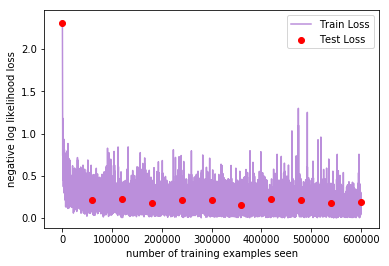
\includegraphics[width=.5\linewidth]{mlp.png}}
        \hfill
        \subfloat[Modelo CNN.]{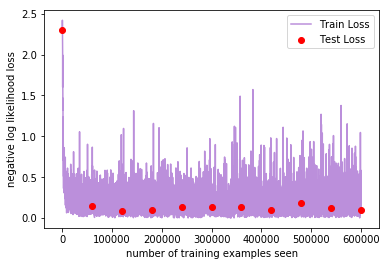
\includegraphics[width=.5\linewidth]{cnn.png}}
        \caption{Curva de aprendizado dos melhores modelos de cada tipo de arquitetura.}
        \label{fig:lc}\par}
  \end{figure}



\begin{table}[H]
\caption{Modelos finais avaliados no conjunto de teste.}
\centering
    \label{tab:final}
\large
\begin{tabular}{@{}lll@{}}
\toprule
    Model \fill & Best Epoch  & \hfill  Best Accuracy \\ \midrule
    MLP  &         10  & 0.9663   \\
    CNN  &          7  & 0.9771   \\ \bottomrule
\end{tabular}
\end{table}
    
    \section*{\begin{tcolorbox}
        \huge
        % \headingfont
        \centering
        Conclusões
    \end{tcolorbox}}
    \Large

    O estudo mostrou que tanto a arquitetura MLP como a CNN são viáveis para o problema de classificação de dígitos escritos a mão ~\cite{mnist}. O modelo final de rede convolucional apresentou um resultado ligeiramente melhor -- acurácia de 97.7\% em comparação à 96.6\% referente à MLP.

    O uso de dropout teve pouca influência em ambas as arquiteturas, sendo que nas redes MLP o mesmo contribuiu negativamente para o aumento da acurácia e nas redes CNN um dropout de 30\% foi o que proveu o maior índice. Nas redes MLP a variação do número de neurônios nas camadas intermediárias teve pouca influência o problema pode ser resolvido por modelos mais simples.

    
    \section*{\begin{tcolorbox}
        \huge
        % \headingfont
        \centering
        Agradecimentos
    \end{tcolorbox}}
    \Large

    O estudante gostaria de expressar seu agradecimento ao programa PIBIC/CNPq/Unicamp pelo auxílio financeiro e em especial à Romis Attux por todo o incentivo e apoio durante o desenvolvimento da pesquisa.

    

    \noindent
    \rule{.33\linewidth}{2pt}

{\large
\begin{thebibliography}{9}
    \bibitem{Goodfellow16}
        I. Goodfellow, Y. Bengio, A. Courville.
        \textit{Deep Learning}.
        MIT Press, 2016.
    \bibitem{mnist}
        Y. LeCun.
        \textit{The MNIST Database of Handwritten Digits}.
        \url{http://yann.lecun.com/exdb/mnist}.
        (acessado em 07/07/2019).
    \bibitem{github}
        R. Gonçalves.
        \textit{mnist\_nn}.
        \url{https://github.com/RafaelGoncalves8/mnist_nn}
        (acessado em 20/07/2019).
    \bibitem{nnsvg}
        LeNail.
        \textit{NN-SVG: Publication-Ready Neural Network Architecture Schematics}.
        \url{http://alexlenail.me/NN-SVG/}.
        Journal of Open Source Software, 2019.
        (acessado em 20/07/2019).
\end{thebibliography}
}
\end{multicols}

\end{document}
